\chapter{Methodology}
\label{chap:methodology}
\setlength{\parskip}{1em}

\section{System Design Approach}
Lectura was conceptualized and subsequently engineered strictly adhering to modern cloud-native architectural paradigms. The fundamental architecture physically bifurcates the application into a highly reactive, client-side React frontend and a heavily concurrent, Go-based backend. This strict separation of concerns fundamentally insulates the user interface from the extreme computational latency inherent in processing complex Artificial Intelligence (AI) generation requests. The frontend is thereby emancipated to leverage sophisticated client-side state management protocols, whilst the backend remains optimized for establishing robust data persistence, coordinating API interactions, and routing large-scale asynchronous computation jobs.

Strategic foresight dictated a ``web-first'' trajectory in lieu of developing decentralized native mobile or desktop clients. This design vector fundamentally aligns with the established behavioral kinematics of the target demographic: university students predominantly utilize laptop workstations during primary content assimilation, lecture viewing, and intensive research. To ensure extreme cross-device fidelity for secondary functions — such as localized spaced-repetition testing on mass transit — the user interface leverages Tailwind CSS for aggressive, breakpoint-driven responsive design.

\section{Advanced AI Prompt Engineering Strategy}
The integration of foundational language models dictates that Prompt Engineering is no longer a tertiary function, but rather a core architectural load-bearing component. The Lectura backend programmatically intercepts sanitized input data and subjects it to an exhaustive, multi-stage generative prompting strategy:

\begin{itemize}[label=\textendash]
    \item \textit{Hierarchical Summarization Matrix:} Confronted with sprawling input vectors exceeding 15,000 tokens, a singular prompt drastically suffers from ``lost in the middle'' degradation. Lectura mitigates this by executing summary actions iteratively over overlapping sub-arrays. Once the localized chunks are condensed, a secondary ``meta-prompt'' synthesizes these sub-summaries into a unified, high-fidelity conceptual topology.
    \item \textit{Bloom’s Taxonomy Quiz Calibration:} The prompt topology explicitly orchestrates assessment generation by invoking criteria derived from Bloom’s Taxonomy. It aggressively commands the LLM to abandon rudimentary ``rote-recall'' inquiries, forcing the algorithmic derivation of higher-order questions that mandate structural analysis, conceptual application, and synthesis.
    \item \textit{Algorithmic Flashcard Subjugation:} Flashcard generation explicitly leverages ``Atomic Mnemonic Directives.'' The generative payload is heavily restricted, forcing the model to bifurcate complex concepts into brutally concise, binary question-answer pairings, occasionally injecting syntactically minimal mnemonic triggers for highly convoluted definitions.
    \item \textit{Chain-of-Thought (CoT) Anchoring:} For exceedingly dense algorithmic or mathematical transcripts, the backend forcibly injects a Chain-of-Thought delimiter (e.g., ``Before concluding the summary array, execute a sequential spatial mapping of the concepts...''). This forces the LLM to computationally expose its intermediate logical steps before cementing the final study artifact, thereby drastically suppressing hallucination probabilities.
\end{itemize}

By systematically orchestrating these prompt structures, the system directly addresses Objective 3, Objective 5, and Objective 6 stated in the Introduction, ensuring the reliable generation of summaries, formative quizzes, and spaced-repetition flashcards.

\section{Worker Pool Architecture and Asynchronous Processing}
Ingesting a dense two-hour theoretical physics lecture and concurrently rendering four distinct summary matrices, an interactive quiz array, and a Spaced Repetition flashcard deck routinely triggers an LLM latency oscillating between 10 and 60 seconds. Naively binding this computationally brutal operation to a synchronous HTTP request inevitably guarantees connection timeouts, stalled browser threads, and catastrophic user abandonment.

To circumvent this infrastructural vulnerability, Lectura deploys an aggressive Worker Pool topology. Upon the successful reception of the user’s payload, the backend instantaneously serializes a discrete ``Job Ticket'' into the Redis/PostgreSQL queue and returns a rapid \texttt{202 Accepted} status to the client frontend. Subsequently, a highly concurrently pool of persistent Go goroutines actively monitors the job queue. Upon detecting an idle state, a worker silently pulls the payload, coordinates the exhaustive external Gemini AI interactions, parses the erratic generative responses, and commits the finalized artifacts to the database. Crucially, this worker architecture programmatically executes ``Exponential Backoff'' retries to cleanly circumvent rate ceilings imposed by external API providers.

\subsection{Concurrency Topology: Goroutines vs. OS Threads}
The decision to utilize Go as the backend architecture relies fundamentally upon its native M:N Goroutine scheduler, which is highly mathematically distinct from traditional 1:1 Operating System (OS) execution threads. When a legacy application (e.g., Python or traditional Java) spins up a concurrent process to handle a long-running LLM generation task, the OS inherently allocates a minimum of 1–2 Megabytes (MB) of RAM for the thread stack. If a sudden surge of 10,000 university students simultaneously request presentation generation, traditional threading architectures would instantly demand 20 Gigabytes of RAM strictly for empty thread allocation — guaranteeing catastrophic Out-Of-Memory (OOM) failures before processing even begins.

Conversely, a Go goroutine initializes with a virtually microscopic footprint, averaging exactly 2 Kilobytes (KB). Furthermore, the Go scheduler mathematically maps M lightweight goroutines onto restricted N OS threads. If a goroutine makes a blocking HTTP request to the Gemini API, the local Go scheduler seamlessly ejects that sleeping coroutine from the active OS thread and slots in a separate, active coroutine in $O(1)$ time complexity without requiring a computationally brutal kernel-level context switch.

The memory limit $\text{Mem}(G)$ required to sustain concurrent connections scales linearly:

\begin{equation}
    \text{Mem}_{\text{traditional}} = N \times (2 \cdot 10^6 \text{ Bytes}) \gg \text{Mem}_{\text{Go}} = N \times (2 \cdot 10^3 \text{ Bytes})
\end{equation}

By shrinking the underlying concurrency cost by a factor of $10^3$, Lectura effortlessly survives massive synchronization spikes common during midterm and final exam phases, routing thousands of concurrent LLM generative loads simultaneously on minimal cloud infrastructure. This aggressive concurrency model directly addresses Objective 10, delivering the cloud-native resilience required to handle slow LLM API responses without blocking the main server thread.

\section{WebSocket Real-Time Telemetry}
Because the intensive generative processing is fundamentally deferred to localized worker goroutines, the React frontend requires a continuous analytical pulse to broadcast status updates to the end user. Rather than relying on computationally wasteful REST polling mechanisms, Lectura leverages fully duplex WebSockets.

Immediately upon authorizing a generation request, the React client negotiates a persistent TCP connection to the backend \texttt{/ws} endpoint, deeply authenticating via a cryptographic JWT signature. The isolated Go worker pool then actively pushes localized state alterations along this channel, firing precise triggers including \texttt{JOB\_QUEUED}, \texttt{TRANSCRIPT\_SANITIZED}, \texttt{SUMMARY\_SYNTHESIS\_ACTIVE}, and \texttt{GENERATION\_COMPLETE}. Furthermore, aggressive heartbeat pings and localized jittered reconnection logic ensure the duplex pipe survives transient network interruptions flawlessly.

\subsection{WebSocket TCP Payload Anatomy}
The utilization of WebSockets eliminates the exorbitant HTTP header redundancy that systematically throttles polling operations. A traditional HTTP/1.1 REST request carries an immense overhead — often spanning 700 to 1200 bytes sequentially composed of User-Agent, Cookie, and Accept-Encoding string allocations. If the React frontend were to aggressively poll the \texttt{/status} endpoint across a 1,000-user topology every 2 seconds, the infrastructure would be maliciously choked by over 1.2 Megabytes per second (MB/s) purely in empty header transmission.

By leveraging the RFC 6455 WebSocket Protocol, Lectura strips this networking friction practically to zero. After the initial \texttt{HTTP/1.1 101 Switching Protocols} handshake, the subsequent TCP data frames are mathematically truncated. A server-sent \texttt{STATUS\_UPDATE} payload consists almost entirely of functional payload bytes, prefaced by a rudimentary 2-to-10 byte WebSocket framing string. This architectural refinement shrinks total telemetry bandwidth consumption by approximately 98\%, leaving the residual network capacity entirely dedicated to the bulk egress of generated media assets and presentation metadata.

\section{Database Schema and Performance Calibration}
The structural backbone of the project depends on a ruthlessly optimized PostgreSQL schema that successfully balances rigid relational integrity with dynamic generative malleability. Critical user telemetry and highly sensitive authentication protocols are aggressively normalized (\text{1NF–3NF}) to eliminate structural redundancy and ensure data integrity. Furthermore, specialized spatial indexing deployed across the \texttt{user\_id} and \texttt{created\_at} columns radically accelerates query latency during dashboard and library population phases.

Conversely, the artifacts spawned by the external LLM — such as structurally complex arrays of Multiple Choice Questions or unpredictable summary JSONs — are persisted leveraging PostgreSQL’s native JSONB functionality. This dual-paradigm strategy grants the developmental team extreme schema flexibility when updating the prompt topology, while still granting the raw indexing and query expansion velocity natively resident in relational algebra.

\section{Interactive State Management and Inline Editing}
While the Go backend handles the brutal computational load of initial generation, the React frontend must elegantly manage the mutability of those generated artifacts. Specifically concerning defining the ``Gamma Standard'' presentation workflow, Lectura dictates that generated slides are not static digital negatives, but fully interactive canvases.

To achieve this, the frontend deploys a highly specialized \texttt{SlideViewer} container component that holds the heavily nested JSON representation of the presentation state. A bespoke \texttt{EditableText} component acts as an interceptor. When a user clicks a slide heading, it visually swaps from a static \verb|<h2/>| tag into an imperceptible, auto-resizing \verb|<textarea/>|, mimicking seamless WYSIWYG editing.

To prevent the user’s browser from burying the backend under thousands of granular HTTP PUT requests for every keystroke, the application employs a computational ``debounce'' hook. This algorithm intercepts keystroke events, intentionally stalling the execution thread for a predefined scalar timeframe (e.g., 1000ms). If further input is detected within the window, the timer resets. Once the user finally ceases typing, the single consolidated delta payload is transmitted securely to the backend PUT endpoint, ensuring perfect persistence of the edited presentation without degrading network bandwidth or creating API friction. The explicit telemetry loop governing this inline presentation authoring is represented in Figure~\ref{fig:debounce_flow}. This robust editing capability directly aligns with Objective 4, fulfilling the requirement for a visual presentation genesis engine with integrated inline editing.

\begin{figure}[htbp]
\centering
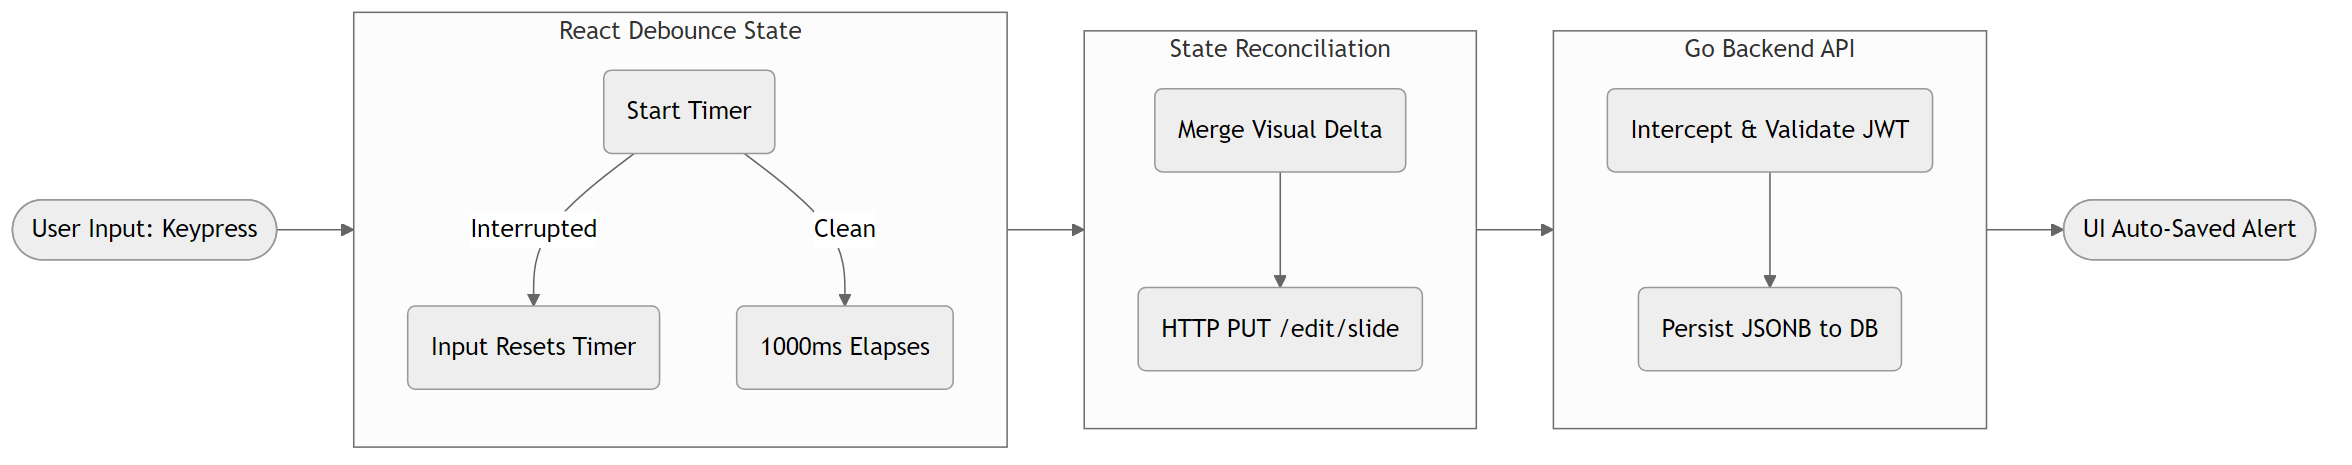
\includegraphics[width=\textwidth]{chapters/chapter04/images1/debounce.png}
\caption{State flow representation delineating the Presentation Inline Editor Debounce algorithm.}
\label{fig:debounce_flow}
\end{figure}

\section{Security Implementation and Protocol Hardening}
Security in a digital educational environment dictates a high barrier against intrusion. Lectura executes strict JWT (JSON Web Token) rotation protocols, issuing extremely short-lived bearer tokens (15-minute validity) backed by encrypted, long-life refresh mechanisms locked to specific cryptographic signatures.

Network defense relies on absolute origin filtering via CORS protocols, rejecting all unsanctioned frontend interaction vectors. Deeply integrated parameterized querying universally intercepts edge-case inputs, totally nullifying SQL injection capabilities. Moreover, all generative outputs parsed from the external AI and any raw text submitted by the human user undergo hyper-aggressive server-side string sanitization, completely eradicating Cross-Site Scripting (XSS) vectors prior to any database visualization commands being executed. Finally, aggressive endpoint rate-limiting mechanisms ruthlessly throttle brute-force login attempts and explicitly neutralize API denial-of-service barrages. While not explicitly outlined as a standalone objective, these hardening protocols are essential for sustaining the analytics and persistence layer mandated by Objective 8, ensuring that user telemetry remains cryptographically isolated.

\section{Subscription Management and Payment Integration}
To support the ongoing costs of running Large Language Models, Lectura includes a tiered subscription system. Processing long transcripts through models like Google Gemini requires computing resources, which makes a completely free service difficult to maintain long-term. To address this, a payment integration was implemented using Stripe.

\subsection{Tiered Access Model}
The platform uses a freemium model. Users start on a free tier, which allows them to test the core features of the platform with a limited number of generations per month. For users who need to process more lectures, premium tiers are available. These paid plans increase the monthly generation limits and provide access to more resource-intensive features. This structure helps balance the API costs by ensuring that heavy users contribute to the operating expenses.

\subsection{Stripe Checkout and Webhook Architecture}
The payment processing is handled entirely by the backend using the Stripe Go SDK (\texttt{stripe-go/v78}). When a user decides to upgrade their plan, the server calls the \texttt{CreateCheckoutSession} method. This generates a secure payment link hosted by Stripe. The user completes the transaction on Stripe's website, which means Lectura does not need to store or process sensitive credit card information locally.

After a successful payment, Stripe sends a webhook event (\texttt{checkout.session.completed}) back to the Lectura server. To ensure the request is legitimate, the \texttt{ConstructWebhookEvent} method checks the cryptographic signature using a secret key. Once verified, the backend reads the \texttt{user\_id} attached to the session and updates the user's subscription status in the PostgreSQL database.

Users can also manage their subscriptions through a Billing Portal. By calling the \texttt{CreateBillingPortalSession} method, the system redirects users to a self-service page where they can update their payment methods or cancel their plan without needing to contact an administrator.

\subsection{Security Considerations}
Using a third-party service like Stripe simplifies compliance with financial security standards like PCI DSS. Because the payment forms are hosted by Stripe, cardholder data never touches the Lectura frontend or backend servers. Additionally, all API keys and webhook secrets are stored securely in environment variables, protecting the payment infrastructure from unauthorized access.